\pdfoptionpdfminorversion=5
\documentclass[9pt,hyperref={pdfpagelabels=false}]{beamer}

\mode<presentation> {
    \usetheme{HHUD}
    \setbeamercovered{invisible}
}

\usepackage[ngerman]{babel}
\usepackage[utf8]{inputenc}
\usepackage{times}
\usepackage[T1]{fontenc}
\usepackage{amsmath}
\usepackage{subfigure}
\usepackage{graphicx}
\usepackage{hyperref}
\usepackage{xmpmulti}
\usepackage{multicol}
\usepackage{appendixnumberbeamer}

% background image
\usebackgroundtemplate{
\includegraphics[width=\paperwidth]{fig/background}}
% commands for low and high decoration in frame foot
\newcommand{\footdecorationlow}{\usebackgroundtemplate{
\includegraphics[width=\paperwidth]{fig/background_small}}}
\newcommand{\footdecorationhigh}{\usebackgroundtemplate{
\includegraphics[width=\paperwidth]{fig/background}}}

% Fix build errors on debian (http://bugs.debian.org/cgi-bin/bugreport.cgi?bug=452333)
\providecommand \thispdfpagelabel[1]{} {}

%% Die folgenden Zeilen können auskommentiert werden, um vor jedem Kapitel eine Gliederungsfolie einzufügen
% \AtBeginSection[] {
%   \footdecorationhigh
%   \begin{frame}<beamer>
%     \thispagestyle{empty}
%     \frametitle{Gliederung}
%     \vspace{-5mm}
%     \tableofcontents[currentsection]
%   \end{frame}
%   \footdecorationlow
% }

% % % % % % % % % %  CHANGE TOPIC AND AUTHOR INFORMATION HERE % % % % % % % % %
\newcommand{\abschluss}{Bachelor}                              % HIER UNZUTREFFENDES LÖSCHEN
\title{\abschluss{}arbeit:\\A Real-time Streaming Protocol for Large-Scale Peer-to-Peer Networks}                      % HIER DEN TITEL DER ARBEIT EINTRAGEN
\author{Christopher Probst}                                                       % HIER DEN NAMEN UND VORNAMEN EINTRAGEN
\date{3.12.2014}                                                                % HIER DAS PRÄSENTATIONSDATUM EINTRAGEN
% % % % % % % % % % % % % % % % % % % % % % % % % % % % % % % % % % % % % % % %
\institute{Institut für Informatik\\Heinrich-Heine-Universität Düsseldorf}
\subject{Informatik}

%
% Hier beginnt das Dokument
%
\begin{document}

  \footdecorationhigh
  \begin{frame}
    \thispagestyle{empty}
    \titlepage
  \end{frame}

  \begin{frame}
    \thispagestyle{empty}
    \frametitle{Gliederung}
    \vspace{-5mm}
    \tableofcontents
  \end{frame}
  \footdecorationlow

  % % % % % % % % % % Ab hier werden die LaTeX-Dateien der einzelnen Abschnitte eingefügt % % % % % % % % % %

  %!TEX root = master.tex

\section{Einleitung}

\subsection{Problemstellung}
\subsection{Motivation}
\subsection{Zielsetzung}

\begin{frame}
  \frametitle{Problemstellung}
	
  \setbeamertemplate{itemize items}[circle]
  \begin{itemize}
	  \item Möchte man Daten von einem einzelnen Computer aus zu beliebig vielen anderen Computern transferieren, so wird häufig ein Client\,/\,Server Netzwerk genutzt. 
	  \item Diese Methode ist einfach, zuverlässig und lang erprobt. Jedoch gibt es Skalierungsprobleme:

 	  \setbeamertemplate{itemize items}[default]
	  \begin{itemize}
	    \item Jeder Client erhöht die Last des Servers
	    \item Mehr Clienten benötigen mehr Server und mehr Bandbreite
	    \item Uploadbandbreite der Clienten bleibt genutzt
	 
	  \end{itemize}
  \end{itemize}
\end{frame}


\begin{frame}
  \frametitle{Motivation}

  \setbeamertemplate{itemize items}[circle]
  \begin{itemize}
	  \item Um ohne ein skalierbares Serversystem Daten dennoch schnell zu verbreiten, kann ein Peer-to-Peer Netzwerk benutzt werden, wo jeder Computer einen Peer darstellt und bei der Datenverbreitung hilft. Einige Anwendungsfälle sind:

	  \setbeamertemplate{itemize items}[default]
	  \begin{itemize}
	    \item File Sharing (BitTorrent)
	    \item Audio und Video Streaming (Skype)    
	    \item DHTs (Kademlia, Chord)
	  \end{itemize}

	  \setbeamertemplate{itemize items}[circle]
	  \item Geräte mit einer geringen Uploadbandbreite können so dennoch schnell Daten verbreiten, wie z.B. ein Live-Videostream von einem Smartphone aus.
  \end{itemize}
\end{frame}


\begin{frame}
  \frametitle{Zielsetzung}

  \setbeamertemplate{itemize items}[circle]

      Implementierung einer Peer-to-Peer Anwendung, die Daten ausgehend von einem Peer, auch genannt Super-Peer, an beliebig viele Peers versendet. Dabei sollen folgende Bedingungen eingehalten werden:

	  \begin{itemize}
	    \item Möglichst hohe Auslastung der Uploadbandbreite der einzelnen Peers.
	    \item Jeder Peer soll die Daten möglichst zur gleichen Zeit fertigstellen.
	    \item Gesamtdauer unabhängig von der Anzahl der Peers.
	    \item Gesamtdauer kleiner als $2 * T_0$.
	  \end{itemize}

\end{frame}



% \begin{frame}
%   \frametitle{Motivation}

%   Sehr praktisch ist die Verwendung von Blöcken:
%   \begin{block}{Normaler Blocktitel}
%     Blöcke sind zur Hervorhebung gedacht. In normalen Blöcken können
%     wichtige Erkenntnisse (Zwischenergebnisse) stehen, die nicht
%     unbemerkt bleiben dürfen.
%   \end{block}

%   \begin{exampleblock}{Beispiel-Blocktitel}
%     Diese Blöcke sind für Beispiele o.ä. gedacht.
%   \end{exampleblock}

%   \begin{alertblock}{Alarm-Blocktitel}
%     Diese Blöcke beinhalten für gewöhnlich Problembeschreibungen.
%   \end{alertblock}
% \end{frame}

% \begin{frame}
%   \frametitle{Weitere Hilfen}

%   Es gibt viele Quellen, die für \LaTeX Beamer herangezogen werden können. Besonders gut sind:
%   \begin{itemize}
%     \item Der Beamer User Guide von Till Tantau:\\\texttt{http://www.math.binghamton.edu/erik/beameruserguide.pdf}
%     \item Ein sehr gutes Beamer Tutorial von Ki-Joo Kim:\\\texttt{http://saikat.guha.cc/ref/beamer\_guide.pdf}
%     \item Der jeweilige Betreuer der Abschlussarbeit :-)
%   \end{itemize}

% \end{frame}


  %!TEX root = master.tex

\section{Umsetzung}

\subsection{Theorie}
\subsection{Implementierung}

\begin{frame}
  \frametitle{Theorie}

  \setbeamertemplate{itemize items}[circle]
  \begin{itemize}  
    \item Die Daten werden vor dem Transfer in kleine Teile (Chunks) geteilt. Es muss mindestens so viele Chunks geben, wie es Peers im Netzwerk gibt.

    \item Der Super-Peer verschickt disjunkte Chunks parallel an alle übrigen Peers.

    \item Jeder Peer verschickt seinen Chunk an alle anderen Peers.

    \item Es wird vereinfacht angenommen, dass jeder Peer die gleiche Uploadbandbreite hat.
  \end{itemize}	

\end{frame}




\begin{frame}
  \frametitle{Theorie}
  Wenn es genauso viele Chunks wie Peers gibt, kann man den Transfer in zwei Stufen betrachten. Peer 1 ist in diesem Fall der Super-Peer.
  \begin{itemize}
    \item Links: Alle Peers bekommen einen disjunkten Chunk vom Super-Peer. 
    \item Rechts: Die Peers schicken sich ihren eigenen Chunk gegenseitig zu. 
  \end{itemize}

  \begin{center}
    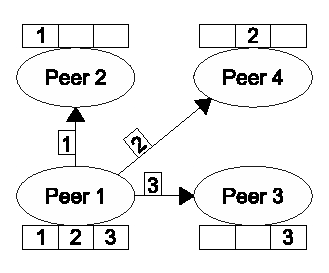
\includegraphics[width=0.4\textwidth]{fig/chunkedswarmmodel1.eps}
    \hspace{0.15\textwidth}
    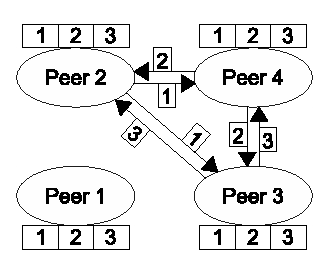
\includegraphics[width=0.4\textwidth]{fig/chunkedswarmmodel2.eps}
  \end{center}
\end{frame}


\begin{frame}
  \frametitle{Theorie}
  Das folgende Bild zeigt den zeitlichen Ablauf:
  \begin{itemize}
    \item In den ersten $T_0$ Sekunden, schickt der Super-Peer einen disjunkten Chunk an jeden Peer. Jeder Chunk ist daher $\frac{Datengr"o"se}{Anzahl}$ groß.
    \item Anschließend schickt jeder Peer seinen Chunk an die anderen beiden Peers, was $\frac{2}{3} * T_0$ Sekunden dauert.
    \item Nach $T_0 + \frac{2}{3} * T_0$ Sekunden besitzt also jeder Peer die Daten.
  \end{itemize}

  \begin{center}
    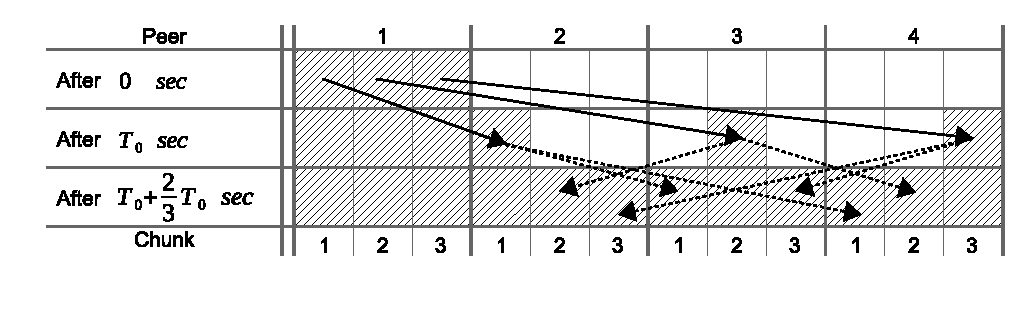
\includegraphics[width=1\textwidth]{fig/chunkedswarmformula1.eps}
  \end{center}
\end{frame}



\begin{frame}
  \frametitle{Theorie}

  \setbeamertemplate{itemize items}[circle]
  \begin{itemize}  
    \item Verdoppelt man die Anzahl der Chunks, halbiert man die Zeit zwischen $T_0$ Sekunden und dem Ende.
    \item Die allgemeine Gesamtdauer lässt sich daher mit $T(n, c) = T_0\:+\:\frac{n}{c}\:*\:\frac{n-1}{n}\:*\:T_0 = (1\:+\:\frac{n-1}{c})\:*\:T_0$ berechnen, wobei $n$ die Anzahl der Peers, jedoch ohne den Super-Peer, und $c = n\:*\:2^i, i \in \mathbb{N}_0$ die Anzahl der Chunks ist.

    \item Mit dieser Methode kann man immer unter $2 * T_0$ Sekunden kommen. Verdoppelt man die Anzahl der Chunks beliebig oft, so kann man sogar beliebig nah an $T_0$ Sekunden herankommen.
  \end{itemize} 

\end{frame}





\begin{frame}
  \frametitle{Implementierung}

  \setbeamertemplate{itemize items}[circle]
  \begin{itemize}  
    \item Mesh Topologie: Jeder Peer ist mit jedem Peer verbunden.
    \item Pull-Based: Chunks werden nur auf Wunsch übertragen.
    \item Announcements: Jeder Peer kündigt an, welche Chunks vorliegen.
    \item Automatic (Re-)Connect: Peers finden andere Peers durch Super-Peer.
  \end{itemize} 

\end{frame}

\begin{frame}
  \frametitle{Implementierung}

  \setbeamertemplate{itemize items}[circle]
  \begin{itemize}  
    \item Peer-Loss Detection: Super-Peer verschickt Chunks von Peers, die das Netzwerk verlassen haben, erneut.
    \item Jeder Peer versucht von möglichst vielen Peers gleichzeitig Chunks zu beziehen. Dies ist wichtig, da ein Pull-Based Ansatz verwendet wird.
    \item Implementiert in Java mit Netty5.
  \end{itemize} 

\end{frame}



  %!TEX root = master.tex

\section{Evaluation}

\subsection{Methodik}
\subsection{Ergebnisse}
\subsection{Fazit}

\begin{frame}
  \frametitle{Theorie}

  \setbeamertemplate{itemize items}[circle]
  \begin{itemize}  
    \item Die Daten werden vor dem Transfer in kleine Teile (Chunks) geteilt. Es muss mindestens so viele Chunks geben, wie es Peers im Netzwerk gibt.

    \item Der Super-Peer verschickt disjunkte Chunks parallel an alle übrigen Peers.

    \item Jeder Peer verschickt seinen Chunk an alle anderen Peers.

    \item Es wird vereinfacht angenommen, dass jeder Peer die gleiche Uploadbandbreite hat.
  \end{itemize}	

\end{frame}



  \appendix

  %!TEX root = master.tex

\section{Anhang}

\subsection{Subsection kann auch leer gelassen werden.}

\begin{frame}
  \frametitle{Sinn des Anhangs}

  In Diskussionen nach Präsentationen kommt es häufiger vor, dass Nachfragen
  gestellt werden, die mit dem regulären Material der Präsentation nicht zu
  beantworten sind.

  Daher lohnt es sich, zusätzliche
  \begin{itemize}
    \item Grafiken
    \item Tabellen mit Detailinformationen
    \item Erklärungen
  \end{itemize}
  aus der schriftlichen Arbeit im Anhang unterzubringen.

\end{frame}


  % % % % % % % % % % Ende der eingefügten LaTeX-Dateien % % % % % % % % % %

\end{document}

%
% Hier endet das Dokument
%